%%%%%%%%%%%%%%%%%%%%%%%%%%%%%%%%%%%%%%%%%
% Jacobs Landscape Poster
% LaTeX Template
% Version 1.0 (29/03/13)
%
% Created by:
% Computational Physics and Biophysics Group, Jacobs University
% https://teamwork.jacobs-university.de:8443/confluence/display/CoPandBiG/LaTeX+Poster
% 
% Further modified by:
% Nathaniel Johnston (nathaniel@njohnston.ca)
%
% This template has been downloaded from:
% http://www.LaTeXTemplates.com
%
% License:
% CC BY-NC-SA 3.0 (http://creativecommons.org/licenses/by-nc-sa/3.0/)
%
%%%%%%%%%%%%%%%%%%%%%%%%%%%%%%%%%%%%%%%%%

%----------------------------------------------------------------------------------------
%	PACKAGES AND OTHER DOCUMENT CONFIGURATIONS
%----------------------------------------------------------------------------------------

\documentclass[final]{beamer}

\usepackage[scale=1.24]{beamerposter} % Use the beamerposter package for laying out the poster

\usetheme{confposter} % Use the confposter theme supplied with this template

\setbeamercolor{block title}{fg=ngreen,bg=white} % Colors of the block titles
\setbeamercolor{block body}{fg=black,bg=white} % Colors of the body of blocks
\setbeamercolor{block alerted title}{fg=white,bg=dblue!70} % Colors of the highlighted block titles
\setbeamercolor{block alerted body}{fg=black,bg=dblue!10} % Colors of the body of highlighted blocks
% Many more colors are available for use in beamerthemeconfposter.sty

%-----------------------------------------------------------
% Define the column widths and overall poster size
% To set effective sepwid, onecolwid and twocolwid values, first choose how many columns you want and how much separation you want between columns
% In this template, the separation width chosen is 0.024 of the paper width and a 4-column layout
% onecolwid should therefore be (1-(# of columns+1)*sepwid)/# of columns e.g. (1-(4+1)*0.024)/4 = 0.22
% Set twocolwid to be (2*onecolwid)+sepwid = 0.464
% Set threecolwid to be (3*onecolwid)+2*sepwid = 0.708

\newlength{\sepwid}
\newlength{\onecolwid}
\newlength{\twocolwid}
\newlength{\threecolwid}
\setlength{\paperwidth}{48in} % A0 width: 46.8in
\setlength{\paperheight}{36in} % A0 height: 33.1in
\setlength{\sepwid}{0.024\paperwidth} % Separation width (white space) between columns
\setlength{\onecolwid}{0.22\paperwidth} % Width of one column
\setlength{\twocolwid}{0.464\paperwidth} % Width of two columns
\setlength{\threecolwid}{0.708\paperwidth} % Width of three columns
\setlength{\topmargin}{-0.5in} % Reduce the top margin size
%-----------------------------------------------------------

\usepackage{graphicx}  % Required for including images

\usepackage{booktabs} % Top and bottom rules for tables

\usepackage[utf8]{inputenc}
\usepackage{subfig, multirow}
\usepackage{tikz, multicol, tabularx}
\usepackage[absolute,overlay]{textpos} 

\graphicspath{{./Images/}}

%----------------------------------------------------------------------------------------
%	TITLE SECTION 
%----------------------------------------------------------------------------------------

\title{Predicting Party Affiliation Using Social Media} % Poster title

\author{Joseph Brown, Mikaela Jordan, and Adam Swayze} % Author(s)

\institute{Tarleton State University} % Institution(s)

%----------------------------------------------------------------------------------------

\begin{document}

\addtobeamertemplate{block end}{}{\vspace*{2ex}} % White space under blocks
\addtobeamertemplate{block alerted end}{}{\vspace*{2ex}} % White space under highlighted (alert) blocks

\setlength{\belowcaptionskip}{2ex} % White space under figures
\setlength\belowdisplayshortskip{2ex} % White space under equations

\begin{frame}[t] % The whole poster is enclosed in one beamer frame

\begin{columns}[t] % The whole poster consists of three major columns, the second of which is split into two columns twice - the [t] option aligns each column's content to the top

\begin{column}{\sepwid}\end{column} % Empty spacer column

\begin{column}{\onecolwid} % The first column

%----------------------------------------------------------------------------------------
%	OBJECTIVES
%----------------------------------------------------------------------------------------

%\begin{alertblock}{Objectives}
%
%Lorem ipsum dolor sit amet, consectetur, nunc tellus pulvinar tortor, commodo eleifend risus arcu sed odio:
%\begin{itemize}
%\item Mollis dignissim, magna augue tincidunt dolor, interdum vestibulum urna
%\item Sed aliquet luctus lectus, eget aliquet leo ullamcorper consequat. Vivamus eros sem, iaculis ut euismod non, sollicitudin vel orci.
%\item Nascetur ridiculus mus.  
%\item Euismod non erat. Nam ultricies pellentesque nunc, ultrices volutpat nisl ultrices a.
%\end{itemize}
%
%\end{alertblock}

%----------------------------------------------------------------------------------------
%	INTRODUCTION
%----------------------------------------------------------------------------------------

%\begin{block}{Introduction}
%
%Lorem ipsum dolor \textbf{sit amet}, consectetur adipiscing elit. Sed commodo molestie porta. Sed ultrices scelerisque sapien ac commodo. Donec ut volutpat elit. Sed laoreet accumsan mattis. Integer sapien tellus, auctor ac blandit eget, sollicitudin vitae lorem. Praesent dictum tempor pulvinar. Suspendisse potenti. Sed tincidunt varius ipsum, et porta nulla suscipit et. Etiam congue bibendum felis, ac dictum augue cursus a. \textbf{Donec} magna eros, iaculis sit amet placerat quis, laoreet id est. In ut orci purus, interdum ornare nibh. Pellentesque pulvinar, nibh ac malesuada accumsan, urna nunc convallis tortor, ac vehicula nulla tellus eget nulla. Nullam lectus tortor, \textit{consequat tempor hendrerit} quis, vestibulum in diam. Maecenas sed diam augue.
%
%This statement requires citation \cite{Smith:2012qr}.
%
%\end{block}
\begin{block}{Introduction}
	During primary elections, polls change quickly and are inaccurate.  The polls from the days leading up to the Wisconsin Republican Primary showed changes in the winner within a day of the primary election.  Finding a better way to predict primary elections is the goal of many political statisticians, and some have used social media to visualize which candidate the majority of a county supports. 
	
	The goal of the project is to predict which candidate will win a primary election in a county based on the words used in tweets originating in that county.  Natural language processing is used to make the computer ``understand'' language. Word clouds can be used as a visualization for this goal.  They depict the frequency of word use in a document by size and shading.  The two word clouds shown here (Figures 2 and 3)come from twitter searches for the keywords ``democrat'' and ``republican.''  
	
	\begin{figure}
\begin{multicols}{3}
\footnotesize{\begin{itemize}
	\item ``Bernie''
	\item ``Sanders''
	\item ``Feel the Bern''
	\item ``Bernie2016''
	\item ``I'm with Her''
	\item ``HillaryClinton''
	\item ``Hillary2016''
	\item ``Clinton''
	\item ``Trump''
	\item ``Donald''
	\item ``Make America Great Again''
	\item ``Trump2016''
	\item ``DonaldTrump''
	\item ``Kasich''
	\item ``JohnKasich''
	\item ``Kasich2016''
	\item ``Cruz''
	\item ``TedCruz''
	\item ``Trust Ted''
	\item ``TrusTed''
	\item ``Cruz2016''
\end{itemize}}
\end{multicols}
\caption{Keywords for Twitter Search}
\end{figure}
	\begin{figure}
		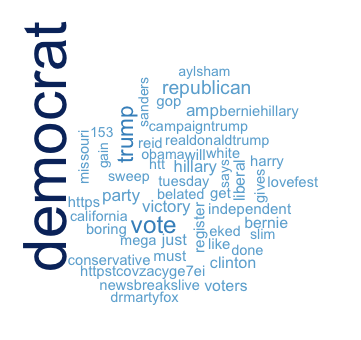
\includegraphics[width=0.45\linewidth]{images/newwordclouddem}
		\caption{Word Cloud for ``Democrat'' Twitter Search}	
	\end{figure}
	\begin{figure}
		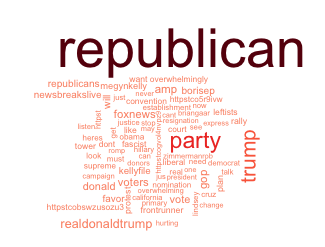
\includegraphics[width=0.45\linewidth]{images/newwordcloudrep}
		\caption{Word Cloud for ``Republican'' Twitter Search}
	\end{figure}



\end{block}

\end{column} % End of the first column

\begin{column}{\sepwid}\end{column} % Empty spacer column

\begin{column}{\twocolwid} % Begin a column which is two columns wide (column 2)

\begin{columns}[t,totalwidth=\twocolwid] % Split up the two columns wide column

\begin{column}{\onecolwid} % The first column within column 2 (column 2.1)

%----------------------------------------------------------------------------------------
%	MATERIALS
%----------------------------------------------------------------------------------------

%\begin{block}{Materials}
%
%The following materials were required to complete the research:
%
%\begin{itemize}
%\item Curabitur pellentesque dignissim
%\item Eu facilisis est tempus quis
%\item Duis porta consequat lorem
%\item Eu facilisis est tempus quis
%\end{itemize}
%
%The materials were prepared according to the steps outlined below:
%
%\begin{enumerate}
%\item Curabitur pellentesque dignissim
%\item Eu facilisis est tempus quis
%\item Duis porta consequat lorem
%\item Curabitur pellentesque dignissim
%\end{enumerate}
%
%\end{block}

%----------------------------------------------------------------------------------------


\begin{block}{Design of Primary Prediction}
The methods of our project can be split into three categories: collecting data, cleaning tweets, and model design.

In order to collect the data, a dataset with the names of all counties in the U.S., the FIPS code for each county (unique identification number for each county in U.S), and the recorded majority winners for each county was created.  A second dataset with the area and centroid of each county was found to set locale for the Twitter search.  The Twitter search encompassed every county in 8 states (Arizona, Florida, Illinois, Indiana, Missouri, North Carolina, Ohio, and Utah).  Twenty-one keywords were included in the search. (Figure 1)

After the Twitter search completed, the dataset with the results from each county was merged with tweets data frame by FIPS code.

When tweets are collected, the resulting document has many impurities in the text.  For ease of analysis, the text is cleaned.  Since the project is based off of term frequency, punctuation is removed and all words are forced into lower case to decrease duplicate terms.  Emojis and stop words (the most common words in the English language) are removed from the text because they will not affect the analysis, and will only make the document term matrices larger. 

For the models, a document-term matrix (DTM) was created from all of the tweets, and a label was attached to each tweet based on the location of the tweet (and which candidate won the Republican and Democrat primary in that county).  Once the DTM was labeled, machine learning algorithms (Support Vector Machine, Artificial Neural Network, and Random Forest) were applied to the data to predict the majority winners of each tweet's county.
\end{block}

\begin{block}{Democrat Results}
	The highest accuracy rates for the democratic party primary predictions were associated with a support vector machine learning algorithm and a neural network with size 6 model.
\end{block}



\end{column} % End of column 2.1




\begin{column}{\onecolwid} % The second column within column 2 (column 2.2)

\begin{block}{Democrat Results Cont'd}
\begin{table}[h!]
\centering
\resizebox{.4\linewidth}{!}{
\begin{tabular}{cc|c|c|}
\cline{3-4}
 & & \multicolumn{2}{|c|}{Predicted} \\
 \cline{3-4}
 & & Bernie & Hillary \\
 \hline
 \multicolumn{1}{|c|}{\multirow{2}{*}{Actual}} & \multicolumn{1}{|c|}{Bernie} & 431 & 3332 \\
 \cline{2-4}
 \multicolumn{1}{|c|}{} & \multicolumn{1}{|c|}{Hillary} & 148 & 10212 \\
 \hline
\end{tabular}}
\caption{SVM Confusion Matrix}
%This model has an accuracy of 75.35934\%
\end{table}
\begin{table}[h!]
\centering
\resizebox{.4\linewidth}{!}{
\begin{tabular}{cc|c|c|}
\cline{3-4}
 & & \multicolumn{2}{|c|}{Predicted} \\
 \cline{3-4}
 & & Bernie & Hillary \\
 \hline
 \multicolumn{1}{|c|}{\multirow{2}{*}{Actual}} & \multicolumn{1}{|c|}{Bernie} & 434 & 3329 \\
 \cline{2-4}
 \multicolumn{1}{|c|}{} & \multicolumn{1}{|c|}{Hillary} & 132 & 10228 \\
 \hline
\end{tabular}}
\caption{Neural Network Confusion Matrix}
%Accuracy rate of 75.49388\%
\end{table}
\begin{table}[h!]
\centering
\resizebox{.4\linewidth}{!}{
\begin{tabular}{c|c}
 & Accuracy Rate \\
 \hline
Support Vector Machine & 75.35934\% \\
\hline
Neural Network & 75.49388\% \\
\end{tabular}}
\caption{Accuracy Rates of Both Models}
\end{table}
Tables 1 and 2 are confusion matrices, and table 3 contains the accuracy rates of both models.  The neural network model has a 0.13\% accuracy rate than the support vector machine model.
\end{block}

\begin{block}{Republican Results}
There are three candidates for the Republican primaries and Trump is winning a far greater number of counties than Cruz and Kasich combined.  Due to those constraints, the models are predicting ``Trump'' or ``not Trump'' rather than each candidate individually. 
\begin{figure}[h!]
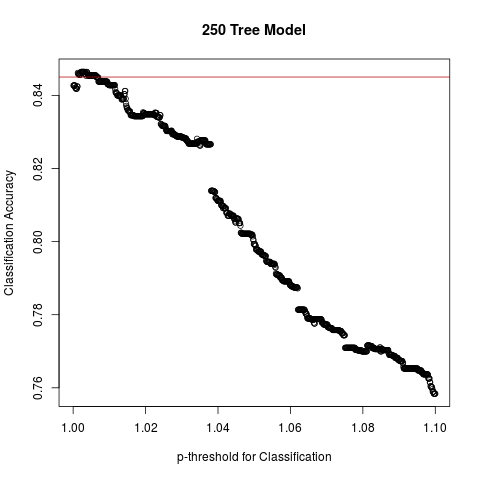
\includegraphics[width=0.25\linewidth]{RFmodelaccuracy250.png}
\caption{Classification accuracy vs Probability threshold}
\end{figure}
\begin{table}
\centering
\resizebox{.4\linewidth}{!}{
\begin{tabular}{cc|c|c|}
\cline{3-4}
 & & \multicolumn{2}{|c|}{Predicted} \\
 \cline{3-4}
 & & Trump & Not Trump \\
 \hline
 \multicolumn{1}{|c|}{\multirow{2}{*}{Actual}} & \multicolumn{1}{|c|}{Trump} & 9517 & 42 \\
 \cline{2-4}
 \multicolumn{1}{|c|}{} & \multicolumn{1}{|c|}{Not Trump} & 1695 & 58 \\
 \hline
\end{tabular}}
\caption{Random Forest 250 Trees Confusion Matrix}
\end{table}

This peak in the graph at .976 shows that in order for the random forest model to predict that a county would go ``not Trump,'' there had to be 97.6\% certainty in that claim (typically this value is set at 50\%).  The model has an accuracy of 84.6\%, only slightly higher than if ``Trump'' was predicted for all counties (84.5\%).

\end{block}


	


\begin{block}{Limitations}
There is a class imbalance issue, as Donald Trump is wining many more precincts than the other Republican candidates.  This skews the model in favor of Trump.  On the Democratic side, a majority of Bernie Sanders supporters are younger and more likely to use Twitter.  According to the Pew Research Center, 88\% of people 21 and younger are active on Twitter.  Some limitations come with the API used to collect tweets, and restrictions from Twitter.  Only 23\% of Americans use Twitter, so the sample might not be representative of the entire population.  Of the tweets that are available, less than 5\% of tweets are georeferenced (which is necessary to be able to label the tweets to train the models).  
	
\end{block}






%----------------------------------------------------------------------------------------
%	METHODS
%----------------------------------------------------------------------------------------

%\begin{block}{Methods}
%
%Lorem ipsum dolor \textbf{sit amet}, consectetur adipiscing elit. Sed laoreet accumsan mattis. Integer sapien tellus, auctor ac blandit eget, sollicitudin vitae lorem. Praesent dictum tempor pulvinar. Suspendisse potenti. Sed tincidunt varius ipsum, et porta nulla suscipit et. Etiam congue bibendum felis, ac dictum augue cursus a. \textbf{Donec} magna eros, iaculis sit amet placerat quis, laoreet id est. In ut orci purus, interdum ornare nibh. Pellentesque pulvinar, nibh ac malesuada accumsan, urna nunc convallis tortor, ac vehicula nulla tellus eget nulla. Nullam lectus tortor, \textit{consequat tempor hendrerit} quis, vestibulum in diam. Maecenas sed diam augue.
%
%\end{block}

%----------------------------------------------------------------------------------------

\end{column}
 % End of column 2.2

%\begin{column}{\sepwid}\end{column} % End of the split of column 2 - any content after this will now take up 2 columns width

%----------------------------------------------------------------------------------------
%	IMPORTANT RESULT
%----------------------------------------------------------------------------------------
%
%\begin{alertblock}{Important Result}
%
%Lorem ipsum dolor \textbf{sit amet}, consectetur adipiscing elit. Sed commodo molestie porta. Sed ultrices scelerisque sapien ac commodo. Donec ut volutpat elit.
%
%\end{alertblock} 

%----------------------------------------------------------------------------------------

%\begin{columns}[t,totalwidth=\twocolwid] % Split up the two columns wide column again

%\begin{column}{\onecolwid} % The first column within column 2 (column 2.1)
%
%%----------------------------------------------------------------------------------------
%%	MATHEMATICAL SECTION
%%----------------------------------------------------------------------------------------
%
%\begin{block}{Mathematical Section}
%
%Nam quis odio enim, in molestie libero. Vivamus cursus mi at nulla elementum sollicitudin. Nam quis odio enim, in molestie libero. Vivamus cursus mi at nulla elementum sollicitudin.
%  
%\begin{equation}
%E = mc^{2}
%\label{eqn:Einstein}
%\end{equation}
%
%Nam quis odio enim, in molestie libero. Vivamus cursus mi at nulla elementum sollicitudin. Nam quis odio enim, in molestie libero. Vivamus cursus mi at nulla elementum sollicitudin.
%
%\begin{equation}
%\cos^3 \theta =\frac{1}{4}\cos\theta+\frac{3}{4}\cos 3\theta
%\label{eq:refname}
%\end{equation}
%
%Nam quis odio enim, in molestie libero. Vivamus cursus mi at nulla elementum sollicitudin. Nam quis odio enim, in molestie libero. Vivamus cursus mi at nulla elementum sollicitudin.
%
%\begin{equation}
%\kappa =\frac{\xi}{E_{\mathrm{max}}} %\mathbb{ZNR}
%\end{equation}
%
%\end{block}
%
%%----------------------------------------------------------------------------------------
%
%\end{column} % End of column 2.1
%
%%\begin{column}{\onecolwid} % The second column within column 2 (column 2.2)
%
%%----------------------------------------------------------------------------------------
%%	RESULTS
%%----------------------------------------------------------------------------------------
%
%\begin{block}{Results}
%
%\begin{figure}
%
\includegraphics[width=0.8\linewidth]{placeholder.jpg}
%\caption{Figure caption}
%\end{figure}
%
%Nunc tempus venenatis facilisis. Curabitur suscipit consequat eros non porttitor. Sed a massa dolor, id ornare enim:
%
%\begin{table}
%\vspace{2ex}
%\begin{tabular}{l l l}
%\toprule
%\textbf{Treatments} & \textbf{Response 1} & \textbf{Response 2}\\
%\midrule
%Treatment 1 & 0.0003262 & 0.562 \\
%Treatment 2 & 0.0015681 & 0.910 \\
%Treatment 3 & 0.0009271 & 0.296 \\
%\bottomrule
%\end{tabular}
%\caption{Table caption}
%\end{table}
%
%\end{block}
%
%%----------------------------------------------------------------------------------------
%
%\end{column} % End of column 2.2
%
\end{columns} % End of the split of column 2
%
\end{column} % End of the second column
%
\begin{column}{\sepwid}\end{column} % Empty spacer column
%
\begin{column}{\onecolwid} % The third column


\begin{block}{Limitations}
There is a class imbalance issue, as Donald Trump is wining many more precincts than the other Republican candidates.  This skews the model in favor of Trump.  On the Democratic side, a majority of Bernie Sanders supporters are younger and more likely to use Twitter.  According to the Pew Research Center, 88\% of people 21 and younger are active on Twitter.  Some limitations come with the API used to collect tweets, and restrictions from Twitter.  Only 23\% of Americans use Twitter, so the sample might not be representative of the entire population.  Of the tweets that are available, less than 5\% of tweets are georeferenced (which is necessary to be able to label the tweets to train the models).  
	
\end{block}



\begin{block}{Future Work}
The models are continuing to be updated as more primary elections occur.  In the future, the models will be improved to account for other geographic differences such as socioeconomic status of precincts.  Debate transcripts will be used in order to predict partiality of media networks using online articles.  The ultimate goal of this project is to extend and improve the current models to predict the outcome of the presidential election this November.
	
\end{block}

\begin{block}{References}
\footnotesize
\noindent Benyamin, Dan.``A Gentle Introduction to Random Forests, Ensembles, \\
\hspace{1cm}and Performance Metrics in a Commercial System - Blog \& Press'' \\ 
\hspace{1cm}\textit{Citizen and Net.} N.p., 09 Nov. 2012. Web. 28 Mar. 2016. \\
Phillips, Winfred.  ``Introduction to Natural Language Processing.'' \\
\hspace{1cm}\textit{Consortium on Cognitive Science Instruction.} The MIND Project,\\
\hspace{1cm}2006.  Web.  16 Mar 2016. \\
Raine, Lee. ``Social Media and Voting." \textit{Pew Research Center Internet} \\
\hspace{1cm}\textit{Science Tech RSS.} Pew Charitable Trusts, 05 Nov. 2012. \\
\hspace{1cm}Web. 28 Mar. 2016. \\
Weston, Jason. ``Support Vector Machines (and Statistical Learning \\
\hspace{1cm}Theory)." ComputerScience4701. Columbia University, New York. \\
\hspace{1cm}\textit{Columbia University}. Web. 28 Mar. 2016.\\
``FiveThirtyEight.'' \textit{FiveThirtyEight.} Nate Silver, n.d. Web.  28 Mar 2016. \\
``2016 Primary Election Results: President Live Map by State, Real-Time \\
\hspace{1cm}Voting Updates'' \textit{Election Hub.}
Politico LLC, 27 Mar. 2016.  Web.  \\
\hspace{1cm}28 Mar. 2016. \\

	
\end{block}



%
%%----------------------------------------------------------------------------------------
%%	CONCLUSION
%%----------------------------------------------------------------------------------------
%
%\begin{block}{Conclusion}
%
%Nunc tempus venenatis facilisis. \textbf{Curabitur suscipit} consequat eros non porttitor. Sed a massa dolor, id ornare enim. Fusce quis massa dictum tortor \textbf{tincidunt mattis}. Donec quam est, lobortis quis pretium at, laoreet scelerisque lacus. Nam quis odio enim, in molestie libero. Vivamus cursus mi at \textit{nulla elementum sollicitudin}.
%
%\end{block}
%
%%----------------------------------------------------------------------------------------
%%	ADDITIONAL INFORMATION
%%----------------------------------------------------------------------------------------
%
%\begin{block}{Additional Information}
%
%Maecenas ultricies feugiat velit non mattis. Fusce tempus arcu id ligula varius dictum. 
%\begin{itemize}
%\item Curabitur pellentesque dignissim
%\item Eu facilisis est tempus quis
%\item Duis porta consequat lorem
%\end{itemize}
%
%\end{block}
%
%%----------------------------------------------------------------------------------------
%%	REFERENCES
%%----------------------------------------------------------------------------------------
%
%\begin{block}{References}
%
%\nocite{*} % Insert publications even if they are not cited in the poster
%\small{\bibliographystyle{unsrt}
%\bibliography{sample}\vspace{0.75in}}
%
%\end{block}
%
%%----------------------------------------------------------------------------------------
%%	ACKNOWLEDGEMENTS
%%----------------------------------------------------------------------------------------
%
%\setbeamercolor{block title}{fg=red,bg=white} % Change the block title color
%
%\begin{block}{Acknowledgements}
%
%\small{\rmfamily{Nam mollis tristique neque eu luctus. Suspendisse rutrum congue nisi sed convallis. Aenean id neque dolor. Pellentesque habitant morbi tristique senectus et netus et malesuada fames ac turpis egestas.}} \\
%
%\end{block}
%
%%----------------------------------------------------------------------------------------
%%	CONTACT INFORMATION
%%----------------------------------------------------------------------------------------
%
%\setbeamercolor{block alerted title}{fg=black,bg=norange} % Change the alert block title colors
%\setbeamercolor{block alerted body}{fg=black,bg=white} % Change the alert block body colors
%
%\begin{alertblock}{Contact Information}
%
%\begin{itemize}
%\item Web: \href{http://www.university.edu/smithlab}{http://www.university.edu/smithlab}
%\item Email: \href{mailto:john@smith.com}{john@smith.com}
%\item Phone: +1 (000) 111 1111
%\end{itemize}
%
%\end{alertblock}
%
%\begin{center}
%\begin{tabular}{ccc}
%
\includegraphics[width=0.4\linewidth]{logo.png} & \hfill & 
\includegraphics[width=0.4\linewidth]{logo.png}
%\end{tabular}
%\end{center}
%
%%----------------------------------------------------------------------------------------
%
\end{column} % End of the third column

\end{columns} % End of all the columns in the poster

\end{frame} % End of the enclosing frame

\end{document}
